% Standard Article Definition
\documentclass[]{article}

% Page Formatting
\usepackage[margin=1in]{geometry}
\setlength\parindent{0pt}

% Graphics
\usepackage{graphicx}

% Math Packages
\usepackage{physics}
\usepackage{amsmath, amsfonts, amssymb, amsthm}
\usepackage{mathtools}

% Extra Packages
\usepackage{pdfpages}
\usepackage{hyperref}
% \usepackage{listings}

% Section Heading Settings
% \usepackage{enumitem}
% \renewcommand{\theenumi}{\alph{enumi}}
\renewcommand*{\thesection}{Problem \arabic{section}}
\renewcommand*{\thesubsection}{\arabic{section}\alph{subsection})}
\renewcommand*{\thesubsubsection}{}%\quad \quad \roman{subsubsection})}

\newcommand{\Problem}{\subsubsection*{\textbf{PROBLEM:}}}
\newcommand{\Solution}{\subsubsection*{\textbf{SOLUTION:}}}
\newcommand{\Preliminaries}{\subsubsection*{\textbf{PRELIMINARIES:}}}

%Custom Commands
\newcommand{\N}{\mathbb{N}}
% \newcommand{\Z}{\mathbb{Z}}
% \newcommand{\Q}{\mathbb{Q}}
\newcommand{\R}{\mathbb{R}}
\newcommand{\C}{\mathbb{C}}

% \newcommand{\SigAlg}{\mathcal{S}}

% \newcommand{\Rel}{\mathcal{R}}

% \newcommand{\toI}{\xrightarrow{\textsf{\tiny I}}}
% \newcommand{\toS}{\xrightarrow{\textsf{\tiny S}}}
% \newcommand{\toB}{\xrightarrow{\textsf{\tiny B}}}

% \newcommand{\divisible}{ \ \vdots \ }
\newcommand{\st}{\ : \ }

% Theorem Definition
\newtheorem{definition}{Definition}
\newtheorem{assumption}{Assumption}
\newtheorem{theorem}{Theorem}
\newtheorem{lemma}{Lemma}
\newtheorem{proposition}{Proposition}
\newtheorem{remark}{Remark}
% \newtheorem{example}{Example}
% \newtheorem{counterExample}{Counter Example}


%opening
\title{
    MECH 6326 - Optimal Control and Dynamic Programming \\ 
    Homework 2
}
\author{Jonas Wagner\\ jonas.wagner@utdallas.edu}
\date{2023, March 3\textsuperscript{rd}}

\begin{document}

\maketitle

\tableofcontents

\newpage
\textbf{Markov Chains}
% Problem 1 ----------------------------------------------
\section{Epidemic model simulation} 
Consider an epidemic model where each individual can be in one of four states: 
susceptible (S), infected (I), deceased (D), or protected (or immune) (P). 
An individual can transition from S to I (they become infected), from I to D (they die), from I to S (they recover, but without immunity), or from I to P (they recover, and now have immunity). 
The states D and P are absorbing: once an individual is in either of these states, they never leave. 
The transition probabilities for each individual are, with infection states ordered (S,I,D,P),
\[
    \mqty[
        0.6 & 0.4 & 0   & 0   \\
        0.2 & 0.6 & 0.1 & 0.1 \\
        0   & 0   & 1   & 0   \\
        0   & 0   & 0   & 1],
\] with an infected neighbor \[
    \mqty[
        1   & 0   & 0   & 0   \\
        0.2 & 0.6 & 0.1 & 0.1 \\
        0   & 0   & 1   & 0   \\
        0   & 0   & 0   & 1],
\] with no infected neighbors.

\Problem
A typical individual has four neighbors: one above, one below, one to the left and one to the right; however, individual on the boundary may be missing one or more of these neighbors.
Use Monte Carlo simulation to estimate the expected number of individuals dead at $T = 50$, for a population of 100 individuals on a 10 x 10 grid, starting from the initial distributions:
\begin{itemize}
    \item Two individuals are infected, one at the (2, 2) location, and the other at the (9, 9) location.
    The rest of the population is susceptible.
    \item Two individuals are infected as above, but there are also eight protected individuals, at the following locations:\[
        (2, 3), (3, 2), (3, 7), (4, 6), (6, 4), (7, 3), (8, 9), (9, 8).
    \]
    (These individuals could be immunized, for example.) 
    All others are susceptible.    
\end{itemize}

\Solution
Let each individual be considered a node in the fully neighbor connected $n \cross n$ square configuration.
For each node $(i,j)$, let the state be defined as $\mathcal{X}_{i,j} = \{S,I,D,P\}$.
Let The two transition matrices for a single node will be defined as 
\[
    P_1 = \mqty[
        0.6 & 0.4 & 0   & 0   \\
        0.2 & 0.6 & 0.1 & 0.1 \\
        0   & 0   & 1   & 0   \\
        0   & 0   & 0   & 1]
    ], \quad P_2 = \mqty[
        1   & 0   & 0   & 0   \\
        0.2 & 0.6 & 0.1 & 0.1 \\
        0   & 0   & 1   & 0   \\
        0   & 0   & 0   & 1]
\]

A node-based interaction can be setup where $P_{i,j} = P_1$ if a neighbor is infected and $P_{i,j} = P_2$ if no neighbor is infected.
The entire system can then be structured as a layered markov chain like structure in $\R^{n\cross n \cross 4}$.
This is written as a neighbor dependent update equation in a function and then ran as many monte calrlo simulations in MATLAB. 
The number dead for each simulation becomes the sum of all in the dead state at $N=50$.

\subsection{}
$E[\sum_{i,j} x_{i,j}^{(3)}] = $


\subsection{}


See attached MATLAB.


\newpage
% Problem 2 ----------------------------------------------
\section{Computing limiting transition matrix power and steady state distributions.}
Consider the following Markov Chain transition graph (self-loops are not shown and can be determined from outgoing edges):
\begin{figure}[h]
    
\end{figure}

\subsection{}
\Problem
Identify and classify the communicating classes as transient, ergodic, absorbing, or periodic.
\Solution



\subsection{}
\Problem
Do transition matrix powers for this chain converge? If so, compute the limiting value $L = \lim_{t \to \infty} P^t$.
\Solution



\subsection{}
\Problem
Do state distributions converge to a unique value for any initial distribution? Compute steady-state distributions for the following initial distribution:
\begin{itemize}
    \item $d_0 = [1,0,\dots,0]$
    \item $d_0 = [0,0,0,1,0,\dots,0]$
    \item $d_0 = [0, 0.5, 0, 0, 0.5, 0, \dots,0]$
\end{itemize}

\Solution








\newpage
% Problem 3 ----------------------------------------------
\section{Absorbing Markov Chains} 
\Problem
You and 7 of your friends find a \$100 bill on the floor. 
No one has change to allow splitting it evenly, so you decide to play a game of chance to divide the money probabilistically. 
You all sit around a table. 
The game is played in turns. 
Each turn, one of three things happens with equal probability: 
the bill can move one position to the left, one position to the right, or the game ends and the person with the bill in front of them wins the game. 
You are the oldest in the group, so the bill starts in front of you. 
What are the chances you win the money?

\Solution
A markov chain can describe the situation.

Let $\mathcal{X} \in \{1,\dots,n\}$ where $n=7$.
Let $d_{k} \in \R^n$ represent the probability that each has the \$100 bill.
For index $i$, $i+1$ is to the right and $i-1$ is to the left, and for $i=0$ the left is $j=n$ and for $i=n$ to the right is $j=0$.

First define three transition matrices to describe each of the operations.
For the cases, $P_w = p_w I_{n}$, $P_r = p_r [p_{i,i+1} = 1, p_{0,n}=1]$, and $P_l = p_l [p_{i,i-1} = 1, p_{n,0}=1]$.

When $P_w$ is enacted, the state enters an absorbing state, thus this can be described in many ways, but one involves instead having an augmented the states to be $d_{k} \in \R^{2n}$ and the states $\mathcal{X}^\infty \{n+1, \dots, 2n\}$ are absorbing states relating to winning the event.

For the augmented transition matrix the absorbing states is updating as $\vb{I}_n$, and the resultant transition matrix for the entire markov chain is defined by:\[
    P = \mqty[
        P_{l,r} &  P_w\\
        \vb{0}_n & \vb{I}_n
    ]
\] and since $p_{w} = p_{r} = p_{l} = \frac{1}{3}$,
\[
    P_{l,r} = \qty(P_r + P_l) 
    = \frac{1}{3} \mqty[
        0 & 1 & 0 & \cdots & 0 & 0 & 1 \\
        1 & 0 & 1 & \cdots & 0 & 0 & 0 \\
        0 & 1 & 0 & \cdots & 0 & 0 & 0 \\
       \ddots &\vdots & \vdots & \ddots & \vdots & \vdots & \vdots \\
        0 & 0 & 0 & \cdots & 0 & 1 & 0 \\
        0 & 0 & 0 & \cdots & 1 & 0 & 1 \\
        1 & 0 & 0 & \cdots & 0 & 1 & 0
    ]
\] and $P_{w} = \frac{1}{3} \vb{I}_n$.

For $n = 7$, this results in:
\[
    P_{l,r} = \frac{1}{3} \mqty[
        0 & 1 & 0 & 0 & 0 & 0 & 1 \\
        1 & 0 & 1 & 0 & 0 & 0 & 0 \\
        0 & 1 & 0 & 1 & 0 & 0 & 0 \\
        0 & 0 & 1 & 0 & 1 & 0 & 0 \\
        0 & 0 & 0 & 1 & 0 & 1 & 0 \\
        0 & 0 & 0 & 0 & 1 & 0 & 1 \\
        1 & 0 & 0 & 0 & 0 & 1 & 0
    ]
\] and $\vb{I}_7$.

The result for the probability at steady-state is given by $L = \lim_{k\to \infty} d_0^T P^{k}$, and since the absorbing states are $(n+1),\cdots,2n$, the probability should end with a vector $d_{\infty} = \mqty[\vb{0}_n \\ p_{i}^{(\infty)} \forall_{i=1,\dots,n}]$.

Out of simplicity, the solution can be approximated as $L \approx P^{100}$ and then \[
    d_0^T L = 
    \mqty[  
        0      \\
        0      \\
        0      \\
        0      \\
        0      \\
        0      \\
        0      \\
        0.4483 \\
        0.1724 \\
        0.0690 \\
        0.0345 \\
        0.0345 \\
        0.0690 \\
        0.1724
    ]
\]
Therefore for $n=7$, the approximation is $P(p_1 = 1) \approx 44.83\%$.

\newpage
% Problem 4 ----------------------------------------------
\section{Hitting Times} 
Consider a Markov Chain with states $\mathcal{X} = \{1,2,3,4\}$.
The transition matrix is \[
    P = \mqty[
        0   & 0   & 0.4 & 0.6 \\
        0.3 & 0   & 0.3 & 0.4 \\
        0   & 0.5 & 0   & 0.5 \\
        0   & 0.7 & 0.3 & 0 
    ]    
\]
Each part below defines a type of hitting time $\tau$.
\Problem
For each part, plot the distribution of $\tau$ given that the chain starts in state $x_0 = 1$, and also determine $P(\tau = 10 \st x_0 = 1)$.
\Solution
One method of obtaining $\tau$ is by augmenting the system with an absorbing state that when reaching a state in $\mathcal{E}$ will be sent to instead of continuing and then 
\[
    P(\tau = k) = \sum_{i \in \mathcal{E}} \sum_{j=1}^{n} p_{i,j}
\]
For each section this can be done using this simple process.

\subsection{}
\Problem
The hitting time $\tau_E$, where $E = \{4\}$.
\Solution
For calculating $\tau_E$, the augmented transition matrix becomes
\[
    P = \mqty[
        0   & 0   & 0.4 & 0.6 & 0\\
        0.3 & 0   & 0.3 & 0.4 & 0\\
        0   & 0.5 & 0   & 0.5 & 0\\
        0   & 0   & 0   & 0   & 1\\
        0   & 0   & 0   & 0   & 1
    ]    
\]

The result for $\tau = 10$ is $P(\tau = 10 \st x_0 = 1) = 0.1\%$
along with the distribution in \autoref{fig:pblm4a}.
\begin{figure}[h]
    \centering
    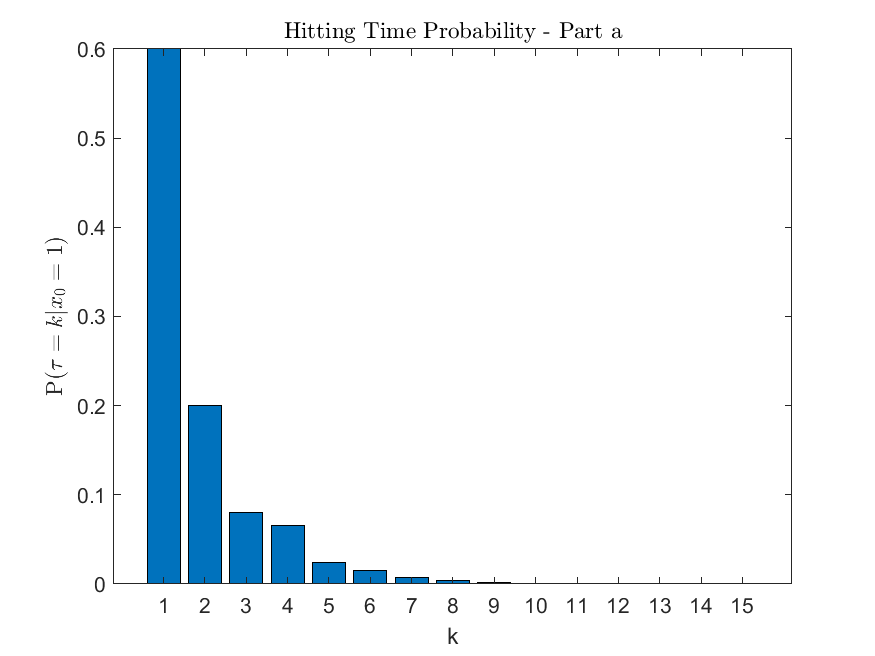
\includegraphics[width = 0.5\textwidth]{figs/pblm4a.png}
    \caption{Distribution for Problem 4a}
    \label{fig:pblm4a}
\end{figure}


\subsection{}
\Problem
The hitting time is the smallest time such that $x_t = 4$ and $x_s = 2$ for some $s < t$, (i.e.) the first time state 4 is visited \emph{after} state 2 has been visited.
\emph{Hint:} Augment the chain with a copy of each state that encodes whether or not state 2 has been visited yet.
\Solution
This problem can be approched in a similar matter; however first the augmented states will be setup to account for when $x_s = 2$.
This would make \[
    P = \mqty[
        0   & 0   & 0.4 & 0.6 & 0   & 0 & 0   & 0   & 0 \\
        0   & 0   & 0   & 0   & 0.3 & 0 & 0.3 & 0.4 & 0 \\
        0   & 0.5 & 0   & 0.5 & 0   & 0 & 0   & 0   & 0 \\
        0   & 0.7 & 0.3 & 0   & 0   & 0 & 0   & 0   & 0 \\
        0   & 0   & 0.4 & 0.6 & 0   & 0 & 0   & 0   & 0 \\
        0.3 & 0   & 0.3 & 0.4 & 0   & 0 & 0   & 0   & 0 \\
        0   & 0.5 & 0   & 0.5 & 0   & 0 & 0   & 0   & 0 \\
        0   & 0   & 0   & 0   & 0   & 0 & 0   & 0   & 1 \\
        0   & 0   & 0   & 0   & 0   & 0 & 0   & 0   & 1
    ]
\]

The result for $\tau = 10$ is $P(\tau = 10 \st x_0 = 1) = 6.62\%$
along with the distribution in \autoref{fig:pblm4b}.
\begin{figure}[h]
    \centering
    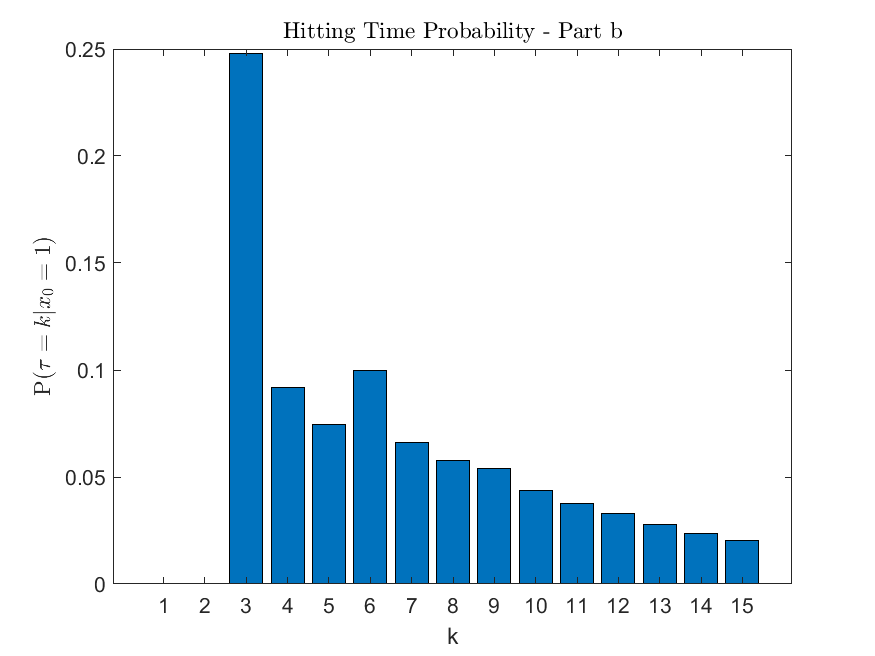
\includegraphics[width = 0.5\textwidth]{figs/pblm4b.png}
    \caption{Distribution for Problem 4b}
    \label{fig:pblm4b}
\end{figure}



\newpage
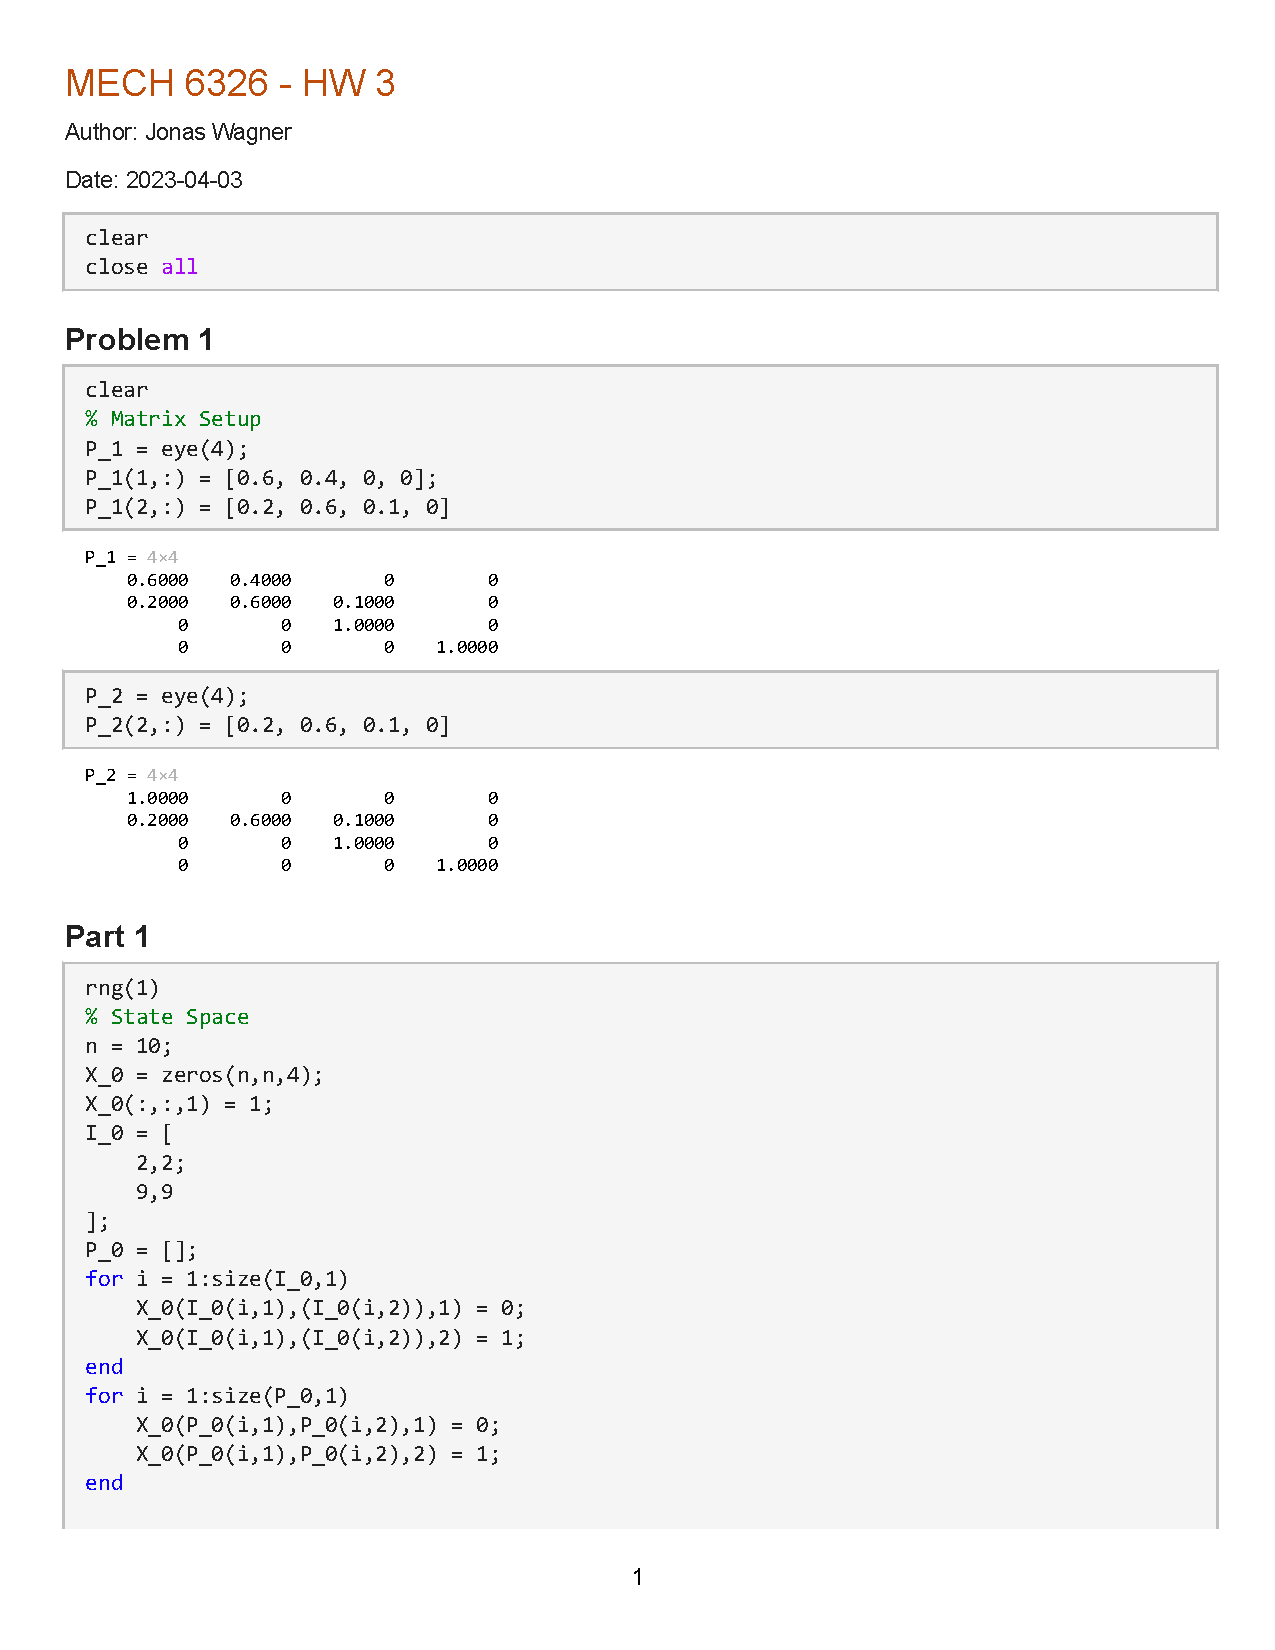
\includepdf[pages=-]{MECH6326_HW3.pdf}

% % Appendix ----------------------------------------------
% \newpage
% \appendix
% \bibliographystyle{plain}
% \bibliography{refs.bib}




\end{document}

